\section{Results}

In this section, the simulation results of NMRAC for a first-order system are presented. The example is constructed, to show that the parameters of the NN converge to the desired values, using the proposed algorithm. The NN consists of one neuron, with an nonlinear actiavtion function, as defined in \eqref{eq:sigmoid}. Hence, the goal of the simulation is to show that $\theta\rightarrow\theta_m$, while keeping all other parameters constant and equal to one another.

The dynamics are chosen to be $a_m=a=10$, $b_m=b=10$, $\theta_m=4$, and the activation function saturates at a value of $1$. The precision threshold $\epsilon$ is chosen to be computer precision in all simulations. We compute the weight update as the analytical solution for each time instance. The sampling time for the simulations is $T_s=0.01$, and the learning rate differs in each simulation to showcase faster and slower convergence. Different simulations for different reference signals are provided, including a constant signal, a sinusodial signal, and a smooth pulse signal. The simluation parameters can be taken from table \ref{tab:sim-settings}.

\begin{table}
    \centering
    \caption{Simulation settings}\label{tab:sim-settings}
    \begin{tabular}{ c c c c } 
            \hline
            & Constant  & Sinusoidal  & Smooth pulse \\
            \hline 
            Learning rate $\gamma$ & 0.05 & 0.15 & 0.005\\ 
            Amplitude & - & 1 & 0.25 \\
            \hline
        \end{tabular}
\end{table}

\subsection{Constant Reference Signal}
\hl{We commence} by using a constant reference signal. We choose the system's initial conditions to be at $0$. The value of the constant reference signal is $1$. This will result in a steady state error for the reference model since we only take a feedback controller into account. However, we will ignore this steady state error, since for us the ability of the controller to learn the behavior of the reference model is of interest. Additionally, we set $\theta_m=4$ and the initial value of the weight $\theta=0$. Finally, we simulate the system response for $5$ seconds and choose the constant parameter $c=0.05$.

In Figure \ref{fig:step}, we observe the steady state error, which is at around $0.2$. As aforementioned, we will disregard this error, since we are interested in how well our NNC can learn the behavior of our reference model. To this end, we can observe that the system converges to the reference model within $5$ seconds. Furthermore, in Figure \ref{fig:step-weights}, we can see the weights of the NNC and the error $e$ are equal to their desired values, $\theta=4$ and $e=0$ respectively. In Figure \ref{fig:Lyapunov-step-input}, we can see that the Lyapunov function converges to zero over time. Additionally, we can see that the derivate of the Lyapunov function is negative and only reaches zero when the Lyapunov function itself converges to zero. This indicates that the proposed learning schematic is stable for the desired reference signal, and we can learn the desired parameter.

\begin{figure}[ht]
    \centering
    \begin{subfigure}[b]{0.49\linewidth}
        \centering
        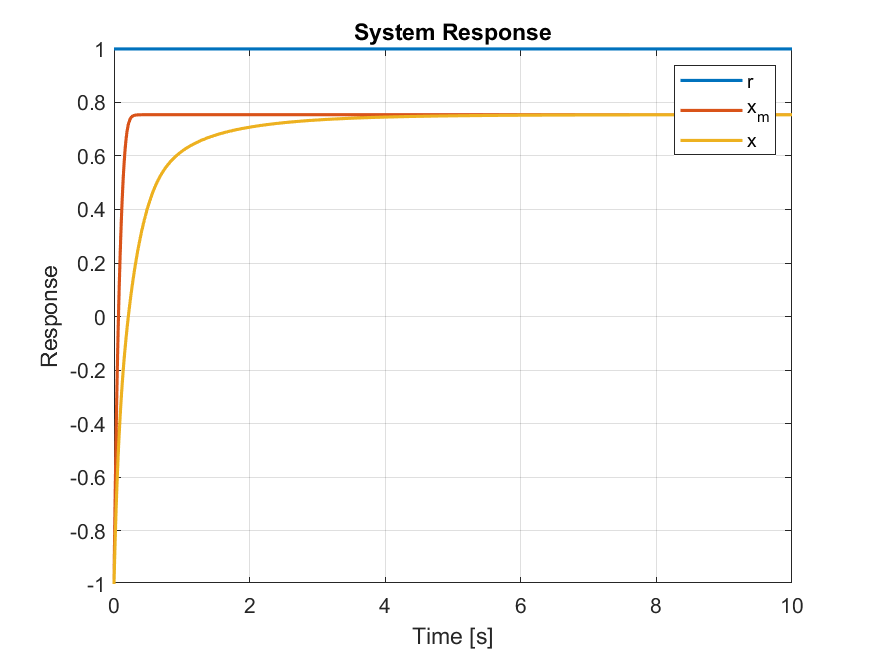
\includegraphics[width=\linewidth]{images/NL-MRAC-SIM/Step/v2/NMRAC_First-Order_Response.png}
        \caption{System response}
        \label{fig:step}
    \end{subfigure}
    \hfill
    \begin{subfigure}[b]{0.49\linewidth}
        \centering
        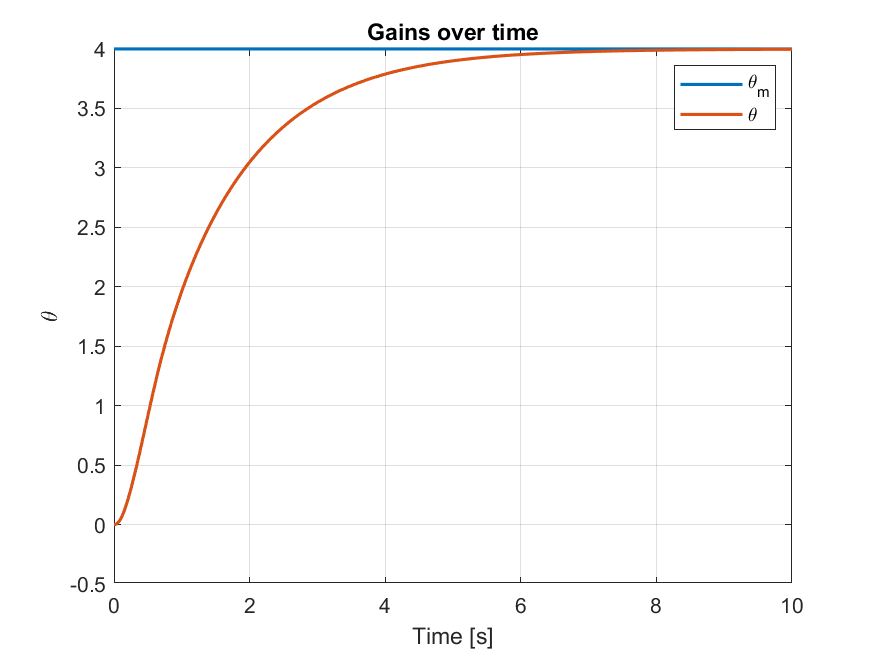
\includegraphics[width=\linewidth]{images/NL-MRAC-SIM/Step/v2/NMRAC_First-Order_Parameters.png}
        \caption{Evolution of gain update}
        \label{fig:step-weights}
    \end{subfigure}
       \caption{Simulation results of nonlinear MRAC with a constant input}
       \label{fig:nl-step}
\end{figure}


\begin{figure}[ht]
    \centering
    \begin{subfigure}[b]{0.49\linewidth}
        \centering
        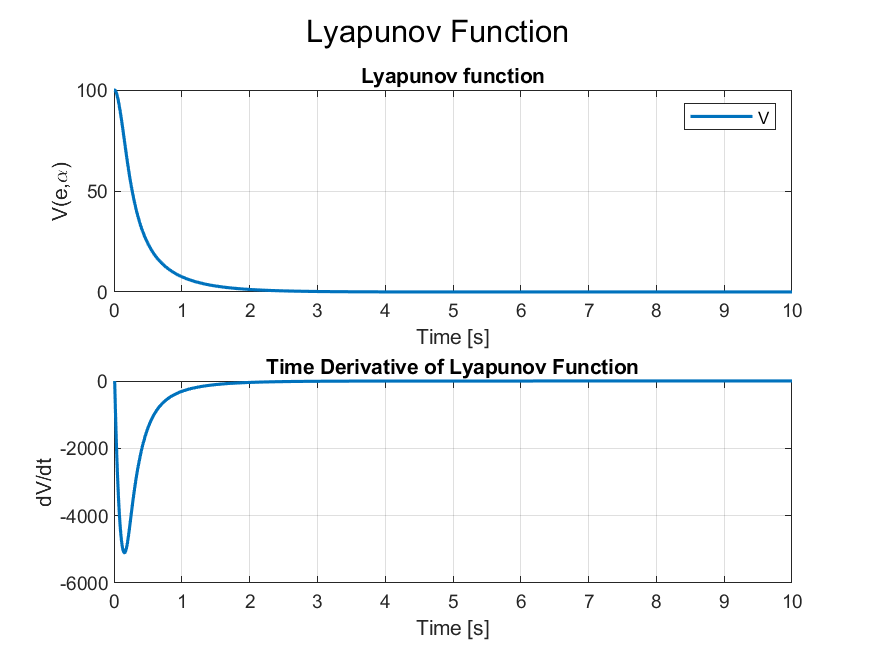
\includegraphics[width=\linewidth]{images/NL-MRAC-SIM/Step/v2/NMRAC_First-Order_Lyapunov.png}
        \caption{Lyapunov function and its time derivate}
        \label{fig:Lyapunov-step-input}
    \end{subfigure}
    \hfill
    \begin{subfigure}[b]{0.49\linewidth}
        \centering
        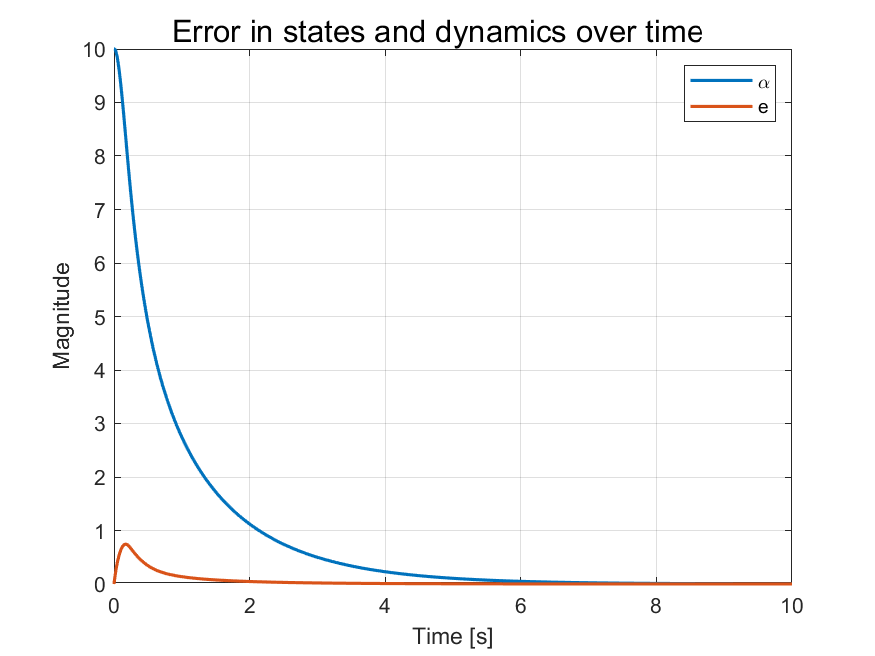
\includegraphics[width=\linewidth]{images/NL-MRAC-SIM/Step/v2/NMRAC_First-Order_Alpha.png}
        \caption{Error in internal states and dynamics of the system}
        \label{fig:step-error}
    \end{subfigure}
       \caption{Lyapunov function and convergence of the system w.r.t. internal states and dynamics}
       \label{fig:step-lyap}
\end{figure}

\subsection{Sine Signal}
\hl{The second} reference is a sinusoid signal, with an amplitude of $0.25$, to stay in a region that is not affected too much by the saturation function. As before, we choose the initial $\theta = 0$, $\theta_m = 4$, and the initial conditions of both the system and the reference model to be at $-1$. We choose this specific initial condition only to be able to see the convergence in the plots. Finally, we simulate the system response for $30$ seconds and choose the constant parameter $c=0.15$, which corresponds to a less aggressive learning strategy compared to the constant input signal.

Figure \ref{fig:sine} shows the response of the system. We observe that the system state, and reference model state both converge towards the desired reference model within around $25$ seconds. Simultaneously, the parameter $\theta$ converges to towards the desired value, which can be seen in Figure \ref{fig:sine-weights}. Even though the parameter converges, we observe oscillations. This behavior is expected, due to the update law. Since the update law is dependent on $\dot e_x$, it is dependent on $\dot r$ and $\dot x$. We observe that whenever $\dot e_x$ switches signs and simultaneously $e$ is small, $\dot \theta$ changes sign, and hence the parameter starts oscillating. This behavior can be changed thourgh adapting the learning rate. A more aggressive learning strategy will be showcased in the next example.

In Figure \ref{fig:Lyapunov-sine-input} we can see that the Lyapunov function converges to zero over time. Additionally, we can see that the derivate of the Lyapunov function is negative and only reaches zero when the Lyapunov function itself converges to zero. The results of this simulation indicate again that the proposed learning schematic is stable for the desired reference signal, and we can learn the desired parameter.

\begin{figure}[ht]
    \centering
    \begin{subfigure}[b]{0.49\linewidth}
        \centering
        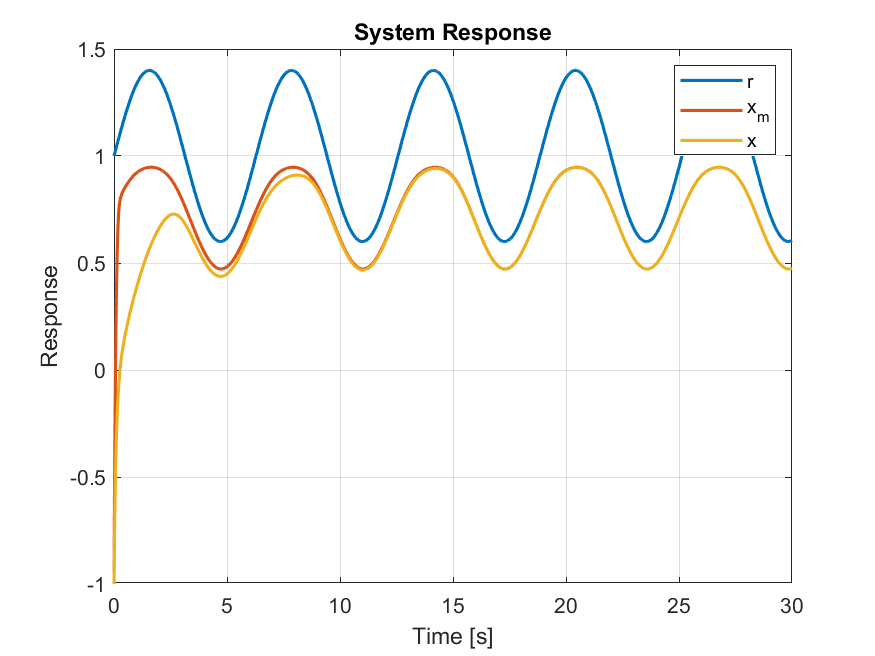
\includegraphics[width=\linewidth]{images/NL-MRAC-SIM/Sine/v2/NMRAC_First-Order_Response.png}
        \caption{System response}
        \label{fig:sine}
    \end{subfigure}
    \hfill
    \begin{subfigure}[b]{0.49\linewidth}
        \centering
        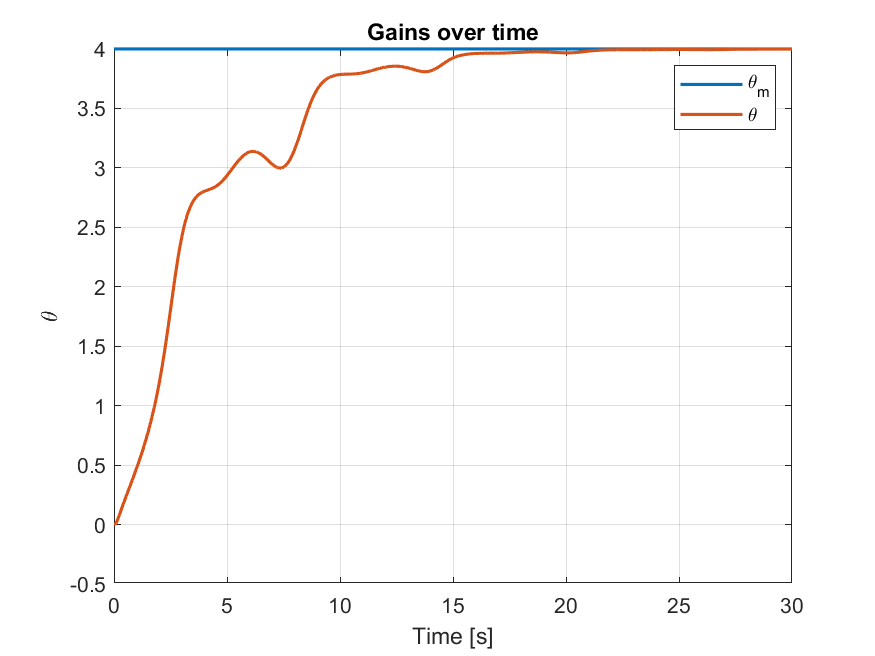
\includegraphics[width=\linewidth]{images/NL-MRAC-SIM/Sine/v2/NMRAC_First-Order_Parameters.png}
        \caption{Evolution of gain update}
        \label{fig:sine-weights}
    \end{subfigure}
       \caption{Simulation results of nonlinear MRAC with a sine input}
       \label{fig:nl-sine}
\end{figure}


\begin{figure}[ht]
    \centering
    \begin{subfigure}[b]{0.49\linewidth}
        \centering
        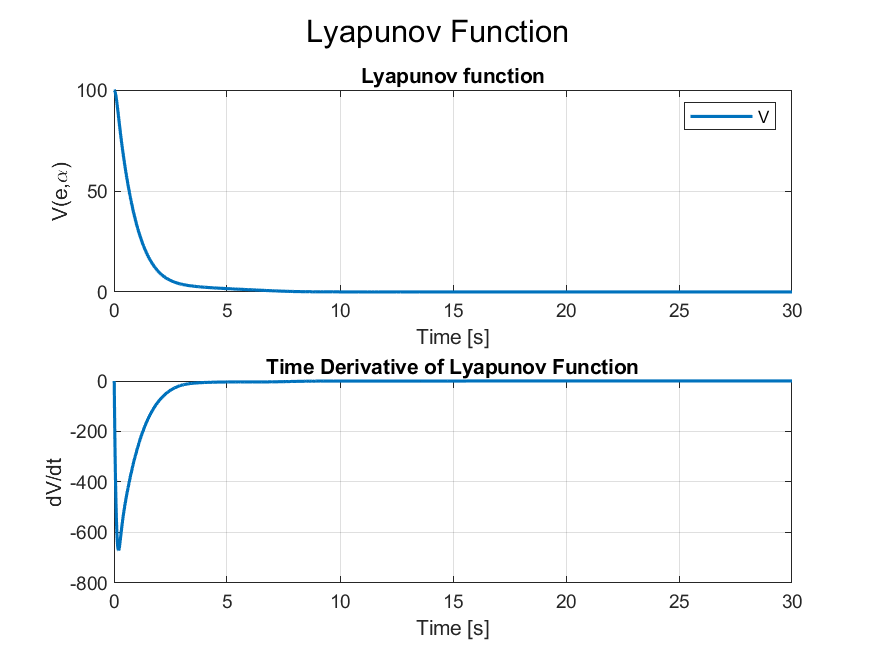
\includegraphics[width=\linewidth]{images/NL-MRAC-SIM/Sine/v2/NMRAC_First-Order_Lyapunov.png}
        \caption{Lyapunov function and its time derivate}
        \label{fig:Lyapunov-sine-input}
    \end{subfigure}
    \hfill
    \begin{subfigure}[b]{0.49\linewidth}
        \centering
        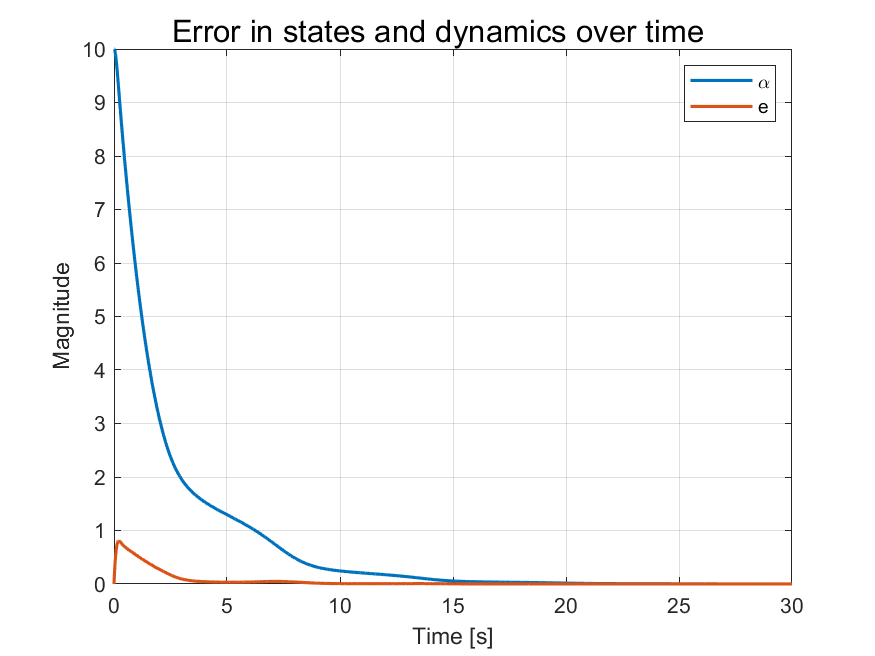
\includegraphics[width=\linewidth]{images/NL-MRAC-SIM/Sine/v2/NMRAC_First-Order_Alpha.png}
        \caption{Error in internal states and dynamics of the system}
        \label{fig:error}
    \end{subfigure}
       \caption{Lyapunov function and convergence of the system w.r.t. internal states and dynamics}
       \label{fig:lyap}
\end{figure}


\subsection{Smooth Pulse Signal}
\hl{The third} and last input signal we will look at is a pulse signal. More specifically, we will use a smooth pulse signal, because we require the reference signal to be continuous since we require its derivative in the update law. We construct the smooth pulse signal, by using a sine function and applying a smooth saturation function, as defined in equation \eqref{eq:sigmoid}. We choose the signal to have an amplitude of $0.25$ and shift the signal such that its minimum value touches upon $0$. As before, we choose the initial conditions of the system and plant to be $-1$. We simulate the system response for $5$ seconds and choose the constant parameter $c=0.005$.

Figure \ref{fig:pulse} shows the response of the system. We can observe that the system converges towards the desired reference model within just under $1$ second. The parameter $\theta$ converges to towards the desired value within $2$ seconds, which can be seen in Figure \ref{fig:pulse-weights}. Even though the parameter converges, we observe that it oscillates. This behavior is expected, due to the update law. Since the update law is dependent on $\dot e_x$, it is dependent on $\dot r$ and $\dot x$. We observe that whenever $\dot e_x$ switches signs and simultaneously $e$ is small, $\dot \theta$ changes sign, and hence the parameter starts oscillating. Similarly, as in the case of the sine input, this behavior can be influenced by decreasing the value of $c$.

The Lyapunov function and its derivative, as shown in Figure \ref{fig:Lyapunov-pulse-input} indicate the convergence of the system and the parameters, since $V$ converges to $0$ and its derivative is always negative and approach zero when $V$ converges. The results of this simulation indicate that the proposed learning schematic is stable for the desired reference signal, and we are able to learn the desired parameter. The three simulation results strongly indicate that with the proposed update law we are able to learn the desired parameters in the presence of a nonlinear activation function.

\begin{figure}[ht]
    \centering
    \begin{subfigure}[b]{0.49\linewidth}
        \centering
        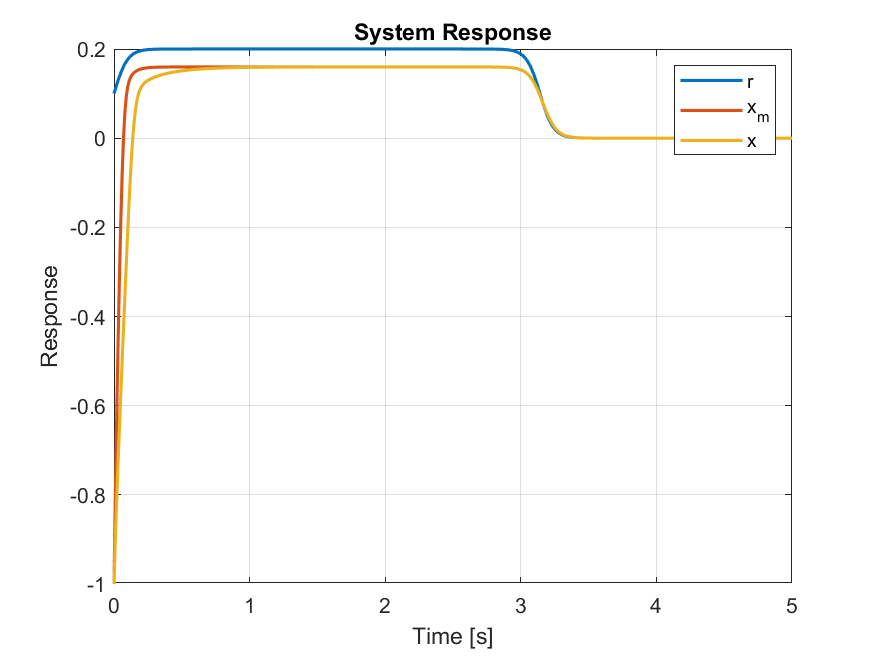
\includegraphics[width=\linewidth]{images/NL-MRAC-SIM/Smooth-Pulse/v2/NMRAC_First-Order_Response.png}
        \caption{System response}
        \label{fig:pulse}
    \end{subfigure}
    \hfill
    \begin{subfigure}[b]{0.49\linewidth}
        \centering
        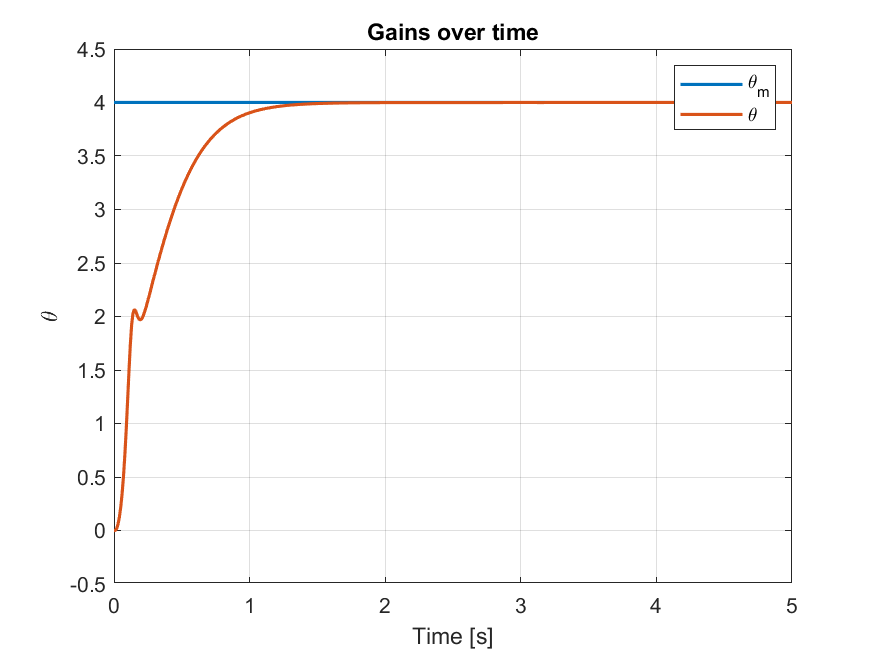
\includegraphics[width=\linewidth]{images/NL-MRAC-SIM/Smooth-Pulse/v2/NMRAC_First-Order_Parameters.png}
        \caption{Evolution of gain update}
        \label{fig:pulse-weights}
    \end{subfigure}
       \caption{Simulation results of nonlinear MRAC with a smooth pulse input}
       \label{fig:nl-pulse}
\end{figure}


\begin{figure}[ht]
    \centering
    \begin{subfigure}[b]{0.49\linewidth}
        \centering
        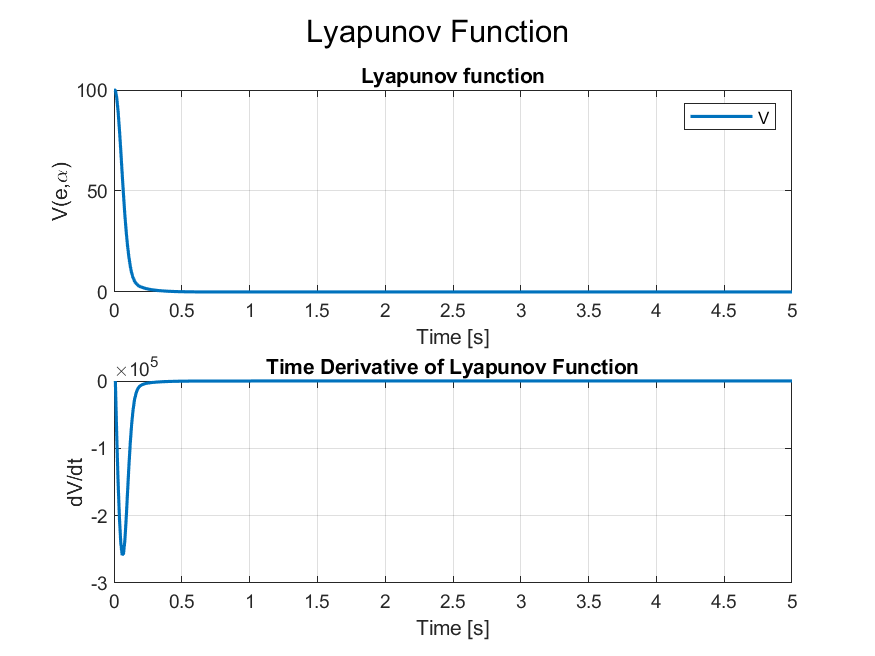
\includegraphics[width=\linewidth]{images/NL-MRAC-SIM/Smooth-Pulse/v2/NMRAC_First-Order_Lyapunov.png}
        \caption{Lyapunov function and its time derivate}
        \label{fig:Lyapunov-pulse-input}
    \end{subfigure}
    \hfill
    \begin{subfigure}[b]{0.49\linewidth}
        \centering
        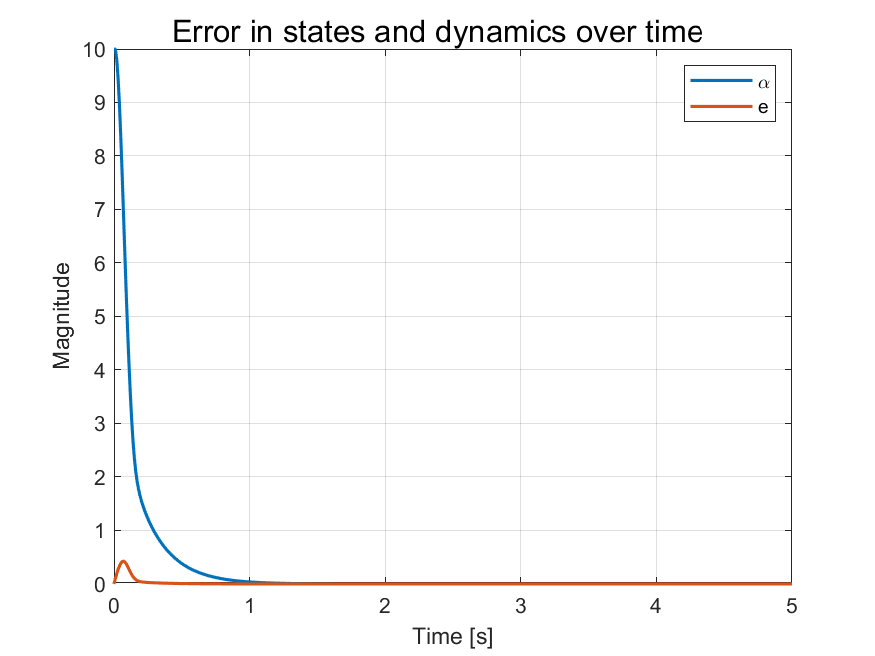
\includegraphics[width=\linewidth]{images/NL-MRAC-SIM/Smooth-Pulse/v2/NMRAC_First-Order_Alpha.png}
        \caption{Error in internal states and dynamics of the system}
        \label{fig:pulse-error}
    \end{subfigure}
       \caption{Lyapunov function and convergence of the system w.r.t. internal states and dynamics}
       \label{fig:pulse-lyap}
\end{figure}